% Options for packages loaded elsewhere
\PassOptionsToPackage{unicode}{hyperref}
\PassOptionsToPackage{hyphens}{url}
\documentclass[
  ignorenonframetext,
]{beamer}
\newif\ifbibliography
\usepackage{pgfpages}
\setbeamertemplate{caption}[numbered]
\setbeamertemplate{caption label separator}{: }
\setbeamercolor{caption name}{fg=normal text.fg}
\beamertemplatenavigationsymbolsempty
% remove section numbering
\setbeamertemplate{part page}{
  \centering
  \begin{beamercolorbox}[sep=16pt,center]{part title}
    \usebeamerfont{part title}\insertpart\par
  \end{beamercolorbox}
}
\setbeamertemplate{section page}{
  \centering
  \begin{beamercolorbox}[sep=12pt,center]{section title}
    \usebeamerfont{section title}\insertsection\par
  \end{beamercolorbox}
}
\setbeamertemplate{subsection page}{
  \centering
  \begin{beamercolorbox}[sep=8pt,center]{subsection title}
    \usebeamerfont{subsection title}\insertsubsection\par
  \end{beamercolorbox}
}
% Prevent slide breaks in the middle of a paragraph
\widowpenalties 1 10000
\raggedbottom
\AtBeginPart{
  \frame{\partpage}
}
\AtBeginSection{
  \ifbibliography
  \else
    \frame{\sectionpage}
  \fi
}
\AtBeginSubsection{
  \frame{\subsectionpage}
}
\usepackage{iftex}
\ifPDFTeX
  \usepackage[T1]{fontenc}
  \usepackage[utf8]{inputenc}
  \usepackage{textcomp} % provide euro and other symbols
\else % if luatex or xetex
  \usepackage{unicode-math} % this also loads fontspec
  \defaultfontfeatures{Scale=MatchLowercase}
  \defaultfontfeatures[\rmfamily]{Ligatures=TeX,Scale=1}
\fi
\usepackage{lmodern}
\ifPDFTeX\else
  % xetex/luatex font selection
\fi
% Use upquote if available, for straight quotes in verbatim environments
\IfFileExists{upquote.sty}{\usepackage{upquote}}{}
\IfFileExists{microtype.sty}{% use microtype if available
  \usepackage[]{microtype}
  \UseMicrotypeSet[protrusion]{basicmath} % disable protrusion for tt fonts
}{}
\makeatletter
\@ifundefined{KOMAClassName}{% if non-KOMA class
  \IfFileExists{parskip.sty}{%
    \usepackage{parskip}
  }{% else
    \setlength{\parindent}{0pt}
    \setlength{\parskip}{6pt plus 2pt minus 1pt}}
}{% if KOMA class
  \KOMAoptions{parskip=half}}
\makeatother
\usepackage{longtable,booktabs,array}
\usepackage{caption}
\captionsetup[table]{skip=6pt}
\newcounter{none} % for unnumbered tables
\usepackage{calc} % for calculating minipage widths
\usepackage{caption}
% Make caption package work with longtable
\makeatletter
\def\fnum@table{\tablename~\thetable}
\makeatother
\usepackage{graphicx}
\makeatletter
\newsavebox\pandoc@box
\newcommand*\pandocbounded[1]{% scales image to fit in text height/width
  \sbox\pandoc@box{#1}%
  \Gscale@div\@tempa{\textheight}{\dimexpr\ht\pandoc@box+\dp\pandoc@box\relax}%
  \Gscale@div\@tempb{\linewidth}{\wd\pandoc@box}%
  \ifdim\@tempb\p@<\@tempa\p@\let\@tempa\@tempb\fi% select the smaller of both
  \ifdim\@tempa\p@<\p@\scalebox{\@tempa}{\usebox\pandoc@box}%
  \else\usebox{\pandoc@box}%
  \fi%
}
% Set default figure placement to htbp
\def\fps@figure{htbp}
\makeatother
\setlength{\emergencystretch}{3em} % prevent overfull lines
\providecommand{\tightlist}{%
  \setlength{\itemsep}{0pt}\setlength{\parskip}{0pt}}
% Auto-generated by infrastructure/rendering/_pdf_latex_helpers.py::extract_math_font_preamble.
% Minimal header passed to Pandoc via -H so Beamer slides pick up the same math font
% as the combined-PDF path. Adjust the manuscript's preamble.md to change the font globally.
\usepackage{unicode-math}
\setmathfont{latinmodern-math.otf}

% Slide layout defaults for warning-clean scientific decks.
\usepackage{etoolbox}
\IfFileExists{xurl.sty}{\usepackage{xurl}}{}
\IfFileExists{seqsplit.sty}{\usepackage{seqsplit}}{\newcommand{\seqsplit}[1]{#1}}
\protected\def\breakseq#1{\seqsplit{#1}}
\protected\def\breaktt#1{\begingroup\ttfamily\seqsplit{#1}\endgroup}
\setlength{\emergencystretch}{6em}
\tolerance=5000
\hbadness=10000
\hfuzz=1pt
\setlength{\tabcolsep}{2pt}
\AtBeginEnvironment{longtable}{\tiny\renewcommand{\arraystretch}{0.86}\setlength{\tabcolsep}{1pt}}
\AtBeginEnvironment{tabular}{\tiny\renewcommand{\arraystretch}{0.86}\setlength{\tabcolsep}{1pt}}
\AtBeginEnvironment{equation}{\tiny}
\AtBeginEnvironment{equation*}{\tiny}
\AtBeginEnvironment{align}{\tiny}
\AtBeginEnvironment{align*}{\tiny}
\AtBeginEnvironment{itemize}{\footnotesize}
\AtBeginEnvironment{enumerate}{\footnotesize}
\AtBeginEnvironment{description}{\footnotesize}
\setbeamerfont{caption}{size=\tiny}
\setbeamerfont{caption name}{size=\tiny}
\setbeamerfont{normal text}{size=\small}
\setbeamerfont{frametitle}{size=\small}
\setbeamerfont{section title}{size=\footnotesize}
\setbeamerfont{subsection title}{size=\footnotesize}
\setbeamertemplate{section page}{%
  \centering
  \begin{beamercolorbox}[sep=12pt,center,wd=\paperwidth]{section title}
    \parbox{0.86\paperwidth}{\centering\usebeamerfont{section title}\insertsection\par}
  \end{beamercolorbox}
}
\setbeamertemplate{subsection page}{%
  \centering
  \begin{beamercolorbox}[sep=8pt,center,wd=\paperwidth]{subsection title}
    \parbox{0.86\paperwidth}{\centering\usebeamerfont{subsection title}\insertsubsection\par}
  \end{beamercolorbox}
}
\setlength{\abovecaptionskip}{2pt}
\setlength{\belowcaptionskip}{0pt}

% Natbib and cross-reference fallbacks — slides don't load natbib
% or cleveref, but combined-PDF manuscript prose may emit these
% commands. The fallback renders citations as a bracketed key list
% and cross-references as detokenized labels so slides don't fail on
% undefined control sequences or raw underscores. \providecommand is
% a no-op if packages load later.
\providecommand{\citep}[1]{[#1]}
\providecommand{\citet}[1]{#1}
\providecommand{\citealp}[1]{#1}
\providecommand{\citeauthor}[1]{#1}
\providecommand{\citeyear}[1]{#1}
\providecommand{\cref}[1]{\texttt{\detokenize{#1}}}
\providecommand{\Cref}[1]{\texttt{\detokenize{#1}}}

\newtheorem{proposition}{Proposition}
\newtheorem{hypothesis}{Hypothesis}
\usepackage{bookmark}
\IfFileExists{xurl.sty}{\usepackage{xurl}}{} % add URL line breaks if available
\urlstyle{same}
% fallback for those not using the hyperref driver hyperxmp:
\makeatletter
\@ifundefined{xmpquote}{\newcommand{\xmpquote}[1]{#1}}{}
\makeatother
\hypersetup{
  hidelinks,
  pdfcreator={LaTeX via pandoc}}

\author{\texorpdfstring{}{}}
\date{}

\begin{document}

\begin{frame}[fragile,allowframebreaks]{Sharp server heuristic:
influence and finite-breakdown characterization}
\protect\phantomsection\label{sec:results-heuristic-characterization}
The server-side \breaktt{robust\_aggregate} rule is the sharp heuristic
axis of the three-axes design (sec.~7.2.1).
It has BH-rejected positive contrasts in the configured accuracy verdict
in sec.~7.5.1 but has declared reversals elsewhere.
Unlike the objective-backed \breaktt{variational\_aggregate}, no
closed-form free-energy derivation has been established for it in this
repository. A separate scoped proposition in the aggregation-objective
supplement rules out the declared continuously differentiable, separable
forward-KL objective class for the implementation's raw log-pool block;
it does not rule out every broader coupled or fixed-point-only
construction. The rule therefore remains a heuristic whose positive
formal property is bit-identical recovery of the log-linear pool at
\breaktt{robustness\ =\ 0} (eq.~7). This section
\end{frame}

\begin{frame}[fragile,allowframebreaks]{Sharp server heuristic:
influence and finite-breakdown characterization}
does not promote the scoped negative result into an objective
certificate; it \emph{measures} the heuristic empirically, and the
measurement makes its honesty boundary concrete.

We measure two things (fig.~\ref{fig:heuristic-breakdown}). First, a
\textbf{numerical influence function}: we drag one agent's belief a
growing fraction toward a confident-wrong contamination point and read
its converged pooling weight. At \breaktt{robustness\ =\ 0} the weight is
a flat \(1/n\) at every perturbation --- the naive pool never
down-weights anyone --- which anchors the instrument to the proven
recovery corner. At positive robustness the dragged agent's influence
falls (not strictly monotonically --- a tiny drag can briefly
\emph{raise} it before the divergence penalty dominates, an honest
non-monotonicity we report rather than smooth away).

\end{frame}

\begin{frame}[fragile,allowframebreaks]{Sharp server heuristic:
influence and finite-breakdown characterization}
Second, and more consequentially, a \textbf{breakdown witness}. We add
colluding confident-wrong adversaries --- all broadcasting the same
false state --- to a fixed colony of 5 honest sentinels until each
aggregator's consensus argmax is \emph{captured} (flips to the
adversaries' target). The sharp heuristic is captured by 2 colluders;
the conservative objective-backed variational rule withstands more,
capitulating only at 4. Both counts are \textbf{finite} (Yes): a
colluding majority overwhelms either rule. That finite breakdown point
is the honest headline: neither rule has an unconditional truth-recovery
claim under coordinated collusion. The absence of an objective theorem
for \breaktt{robust\_aggregate} is a separate derivational boundary, and
the finite capture measurement neither establishes estimator-level
B-robustness nor refutes the variational rule's stated raw
effective-weight result.
\end{frame}

\begin{frame}[fragile,allowframebreaks]{Sharp server heuristic:
influence and finite-breakdown characterization}

The report also runs a declared diagnostic grid over state dimension,
honest-agent count, robustness, four simple attack mechanisms, and
balanced versus adversary-downweighted base weights. This is a coverage
instrument for finding counterexamples, not a random sample of worlds
and not a theorem search over all simplexes. A finite capture row is
evidence against a universal guarantee; an uncaptured row is only ``not
found within this search budget.''

\end{frame}

\begin{frame}[fragile,allowframebreaks]{Sharp server heuristic:
influence and finite-breakdown characterization}
\begin{figure}
\centering
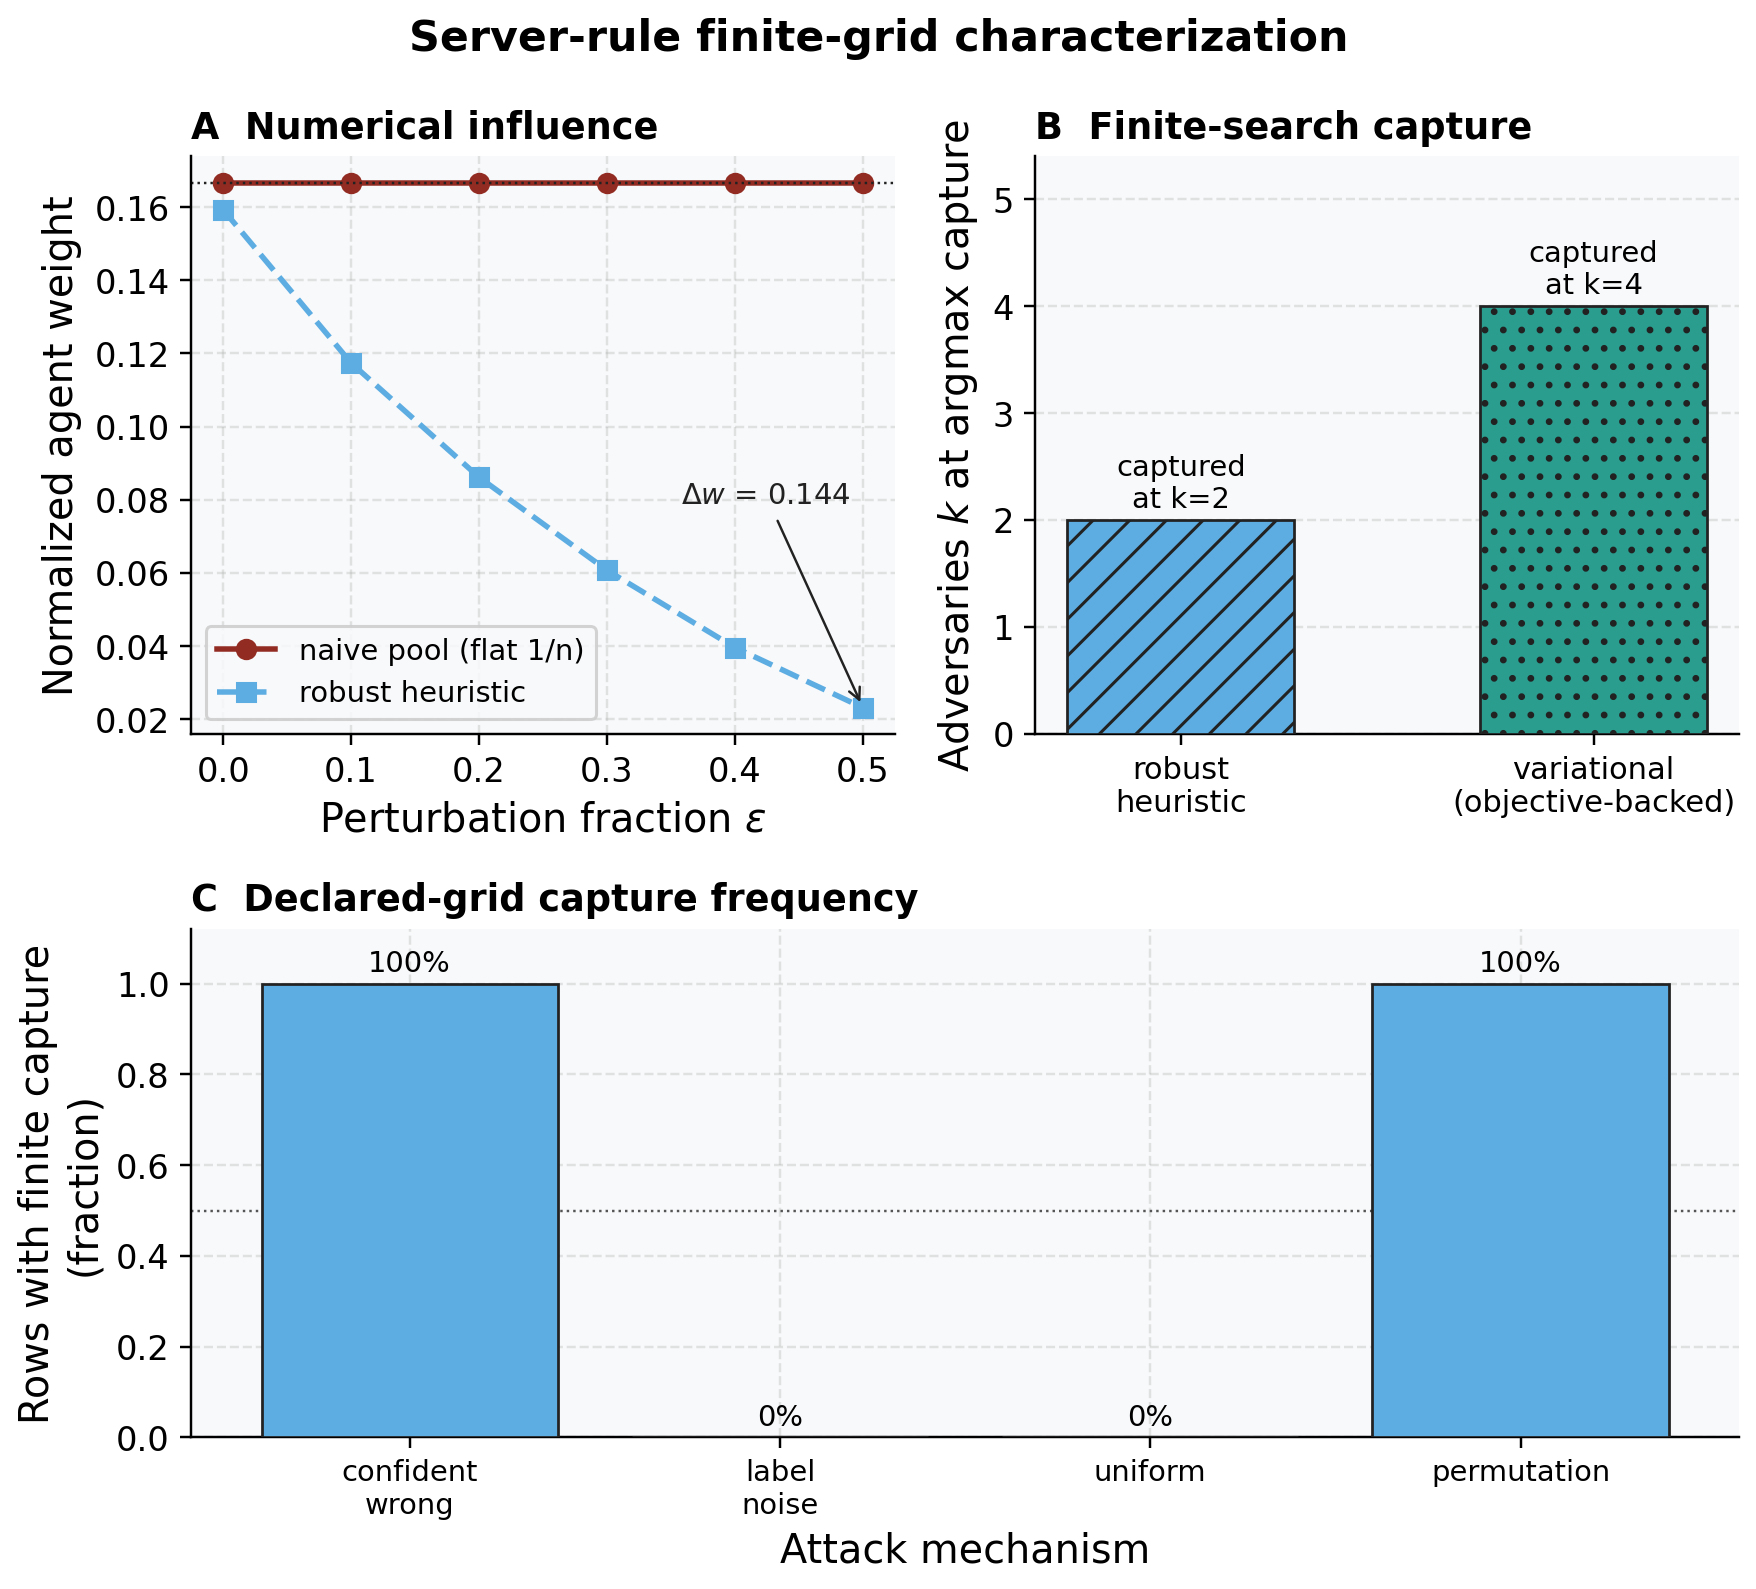
\includegraphics[width=0.95\linewidth,height=0.40\textheight,keepaspectratio,alt={Source relation: original project diagnostic of the server-side heuristic; estimand: numerical influence, finite-search breakdown count, and declared-grid capture fraction; uncertainty: deterministic seeded colonies, so no resampling interval is shown. Empirical characterization of the robust\_aggregate heuristic (two panels plus an optional attack-grid diagnostic). Left panel (numerical influence): the x-axis is the perturbation fraction by which one agent's belief is dragged toward a confident-wrong contamination point; the y-axis is that agent's converged normalized pooling weight, plotted for the naive pool (flat at 1/n, dotted reference) and the robust heuristic (down-weighting). The inset reports the final naive-minus-robust weight gap at the end of the probed path. Labeled ``empirical, at these settings --- not a guarantee.'' Right panel (measured breakdown point): the x-axis is the aggregator (robust heuristic vs objective-backed variational); the y-axis is the number of colluding confident-wrong adversaries that captures that aggregator's consensus argmax --- the robust heuristic at k = 2 and the variational rule at k = 4. Both bars are finite, so neither rule has an unconditional truth-recovery guarantee against coordinated collusion; this does not negate the variational rule's per-agent effective-weight theorem. Deterministic seeded colonies (no resampling), so no error band is applicable. The optional third panel reports the fraction of declared grid rows with finite capture within the configured adversary budget; it is not a probability or a global breakdown bound.}]{../figures/heuristic_breakdown.png}
\caption{Source relation: original project diagnostic of the server-side
heuristic; estimand: numerical influence, finite-search breakdown count,
and declared-grid capture fraction; uncertainty: deterministic seeded
colonies, so no resampling interval is shown. Empirical characterization
of the \protect\breaktt{robust\_aggregate} heuristic (two panels plus an
optional attack-grid diagnostic). Left panel (numerical influence): the
x-axis is the perturbation fraction by which one agent's belief is
dragged toward a confident-wrong contamination point; the y-axis is that
agent's converged normalized pooling weight, plotted for the naive pool
(flat at \(1/n\), dotted reference) and the robust heuristic
(down-weighting). The inset reports the final naive-minus-robust weight
gap at the end of the probed path. Labeled ``empirical, at these
settings --- not a guarantee.'' Right panel (measured breakdown point):
the x-axis is the aggregator (robust heuristic vs objective-backed
variational); the y-axis is the number of colluding confident-wrong
adversaries that captures that aggregator's consensus argmax --- the
robust heuristic at \(k = 2\) and the variational rule at \(k = 4\).
Both bars are finite, so neither rule has an unconditional
truth-recovery guarantee against coordinated collusion; this does not
negate the variational rule's per-agent effective-weight theorem.
Deterministic seeded colonies (no resampling), so no error band is
applicable. The optional third panel reports the fraction of declared
grid rows with finite capture within the configured adversary budget; it
is not a probability or a global breakdown
bound.}\label{fig:heuristic-breakdown}
\end{figure}
\end{frame}

\end{document}
